\documentclass[11pt]{amsart}

\usepackage[a4paper,margin=1in]{geometry}
\usepackage{microtype}
\usepackage{amsmath,amssymb,amsthm,mathtools}
\usepackage{graphicx}
\usepackage{booktabs}
\usepackage[colorlinks=true,linkcolor=blue,citecolor=blue,urlcolor=blue]{hyperref}

\title{Empirical Companion: KL Regularization against an EMA Reference}
\author{Brian Bartoldson}
\date{}

\newcommand{\E}{\mathbb{E}}
\newcommand{\KL}{\mathrm{KL}}

\begin{document}
\maketitle

\begin{abstract}
This note collects empirical results that accompany the theoretical derivation in \texttt{main.tex}. We train Qwen3-4B-Instruct-2507 with TBA on Countdown using asynchronous rollouts ($\Delta=10$) and study three questions: (i) does the first-order EMA-KL approximation track the exact EMA-KL loss closely enough to substitute for it? (ii) Does centering the per-sample KL by a K-group mean help, hurt, or do nothing? (iii) Do the same patterns hold against a periodic-reset reference policy? Across a four-cell matrix, the no-centering cells (both exact and approximate) reach peak eval $0.83$, while the centering cells peak earlier and degrade.
\end{abstract}

\section{Setup}

All runs use Qwen3-4B-Instruct-2507 trained with TBA, $\beta=0.005$, $\alpha=0.9$ EMA decay, $\Delta=\texttt{max\_async\_level}=10$, sampled-$k=$train-$k=16$, sequence length $4096$, learning rate $10^{-6}$, $720$ training steps, evaluation every $20$ steps. The four EMA-reference cells share initialization and only differ in the choices labeled \emph{centering} (per-sample KL minus a K-group mean, vs.\ no centering) and \emph{per-sample KL} (exact $\log T_n - \log E_n$ vs.\ first-order approximation $\frac{\alpha}{\Delta(1-\alpha)}(\log T_n - \log T_{n-\Delta})$ from \texttt{main.tex} eq.~(2.10)).

\section{EMA-reference matrix}

Figure~\ref{fig:ema-matrix} overlays the eval curves for the four cells of the EMA-reference matrix, plus the historical \texttt{klMeanInf\_emaRef} run (which uses the K-group mean of $\log\!\inf - \log E_n$ for centering). Because the live trainer policy and the inference snapshot drift only $\Delta$ steps apart, that "klMeanInf-style" centering term is small in magnitude (we measured the per-sample $\KL$ signed mean as $\sim 9\%$ of the per-sample absolute $\KL$ across this run), so it behaves more like weak no-centering than like a meaningful centering.

\begin{figure}[ht]
  \centering
  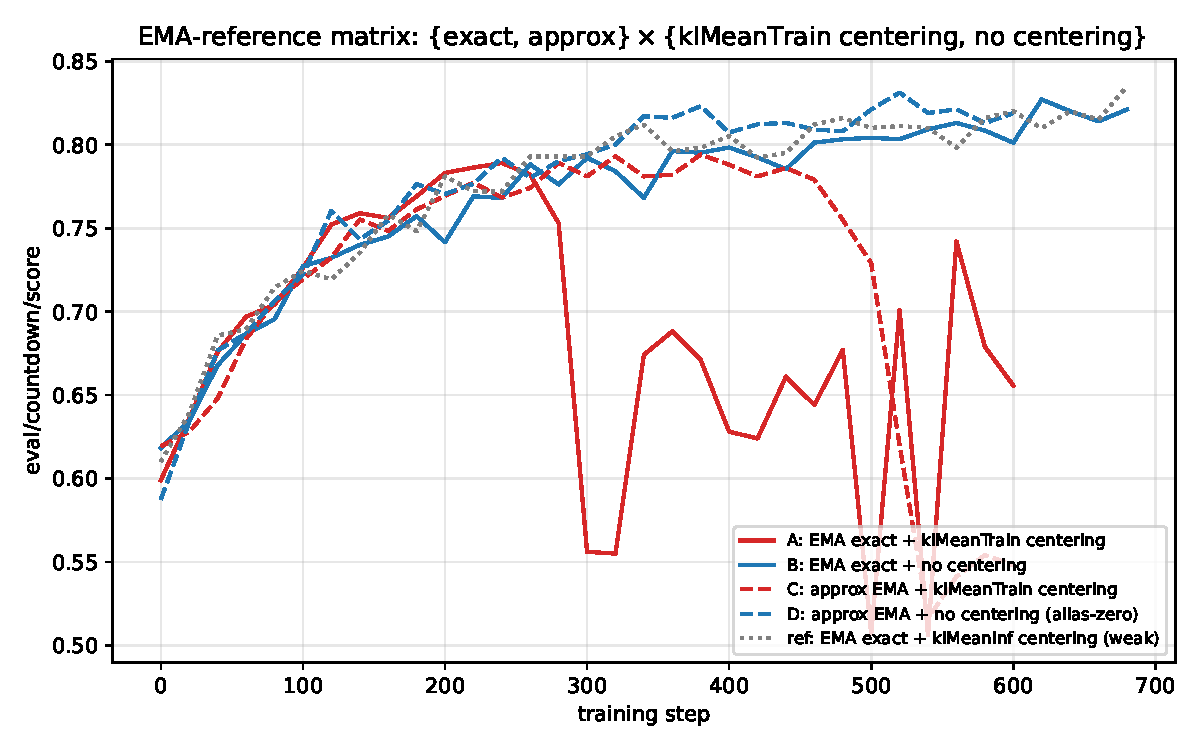
\includegraphics[width=0.95\linewidth]{fig_ema_matrix.pdf}
  \caption{Eval accuracy on Countdown for the four-cell matrix of (per-sample KL, centering) under EMA reference. Solid lines: exact KL; dashed: approx KL. Red: klMeanTrain-style centering; blue: no centering; gray dotted: legacy klMeanInf-style centering, included as reference. Both no-centering cells (B, D) plateau above $0.80$ and peak above $0.83$; both klMeanTrain-style cells (A, C) peak around step $300$ and degrade afterward.}
  \label{fig:ema-matrix}
\end{figure}

\paragraph{Headline numbers.} Peak / final eval (every-20-step Countdown evaluation):
\begin{center}
\begin{tabular}{lccc}
\toprule
Cell & Per-sample KL & K-group mean & Peak (step) / Final \\
\midrule
A: \texttt{emaTrain}        & exact  & klMeanTrain      & $0.789$ (240) / $0.656$ \\
B: \texttt{noCenter}        & exact  & 0 (forced)       & $\mathbf{0.827}$ (620) / $0.821$ \\
C: \texttt{approxUseTrain}  & approx & klMeanTrain      & $0.794$ (380) / $0.548$ \\
D: \texttt{approxUse}       & approx & 0 (alias bug)    & $\mathbf{0.831}$ (520) / $0.819$ \\
\bottomrule
\end{tabular}
\end{center}

\paragraph{Observations.}
\begin{enumerate}[leftmargin=*]
  \item \emph{No centering wins.} Both no-centering cells (B, D) substantially outperform the klMeanTrain-style cells (A, C). klMeanTrain centering subtracts a moving target (mean of $\log T_n - \log E_n$ in case A, mean of $\frac{\alpha}{\Delta(1-\alpha)}(\log T_n - \log\!\inf)$ in case C) that scales with policy drift, and that subtraction destabilizes training around step $300$.
  \item \emph{Approx tracks exact.} B and D produce essentially identical learning curves: peaks $0.827$ vs.\ $0.831$, finals $0.821$ vs.\ $0.819$. The first-order surrogate is a viable replacement for the exact KL when the centering term is held fixed at zero.
  \item \emph{Caveat on cell D.} Cell D was the originally-running \texttt{approxUse} configuration whose K-group mean degenerated to $0$ exactly because of an alias bug between the recompute path and the trainer-forward path; mathematically it equals the explicit no-centering case. We renamed the wandb run to \texttt{noCenterByAlias\_*} to record this.
\end{enumerate}

\section{Reset-reference baseline}

Before the EMA work, the same KL-source $\times$ IS grid was run against a periodic-reset reference (every $50$ steps). Figure~\ref{fig:reset-baselines} shows those eval curves.

\begin{figure}[ht]
  \centering
  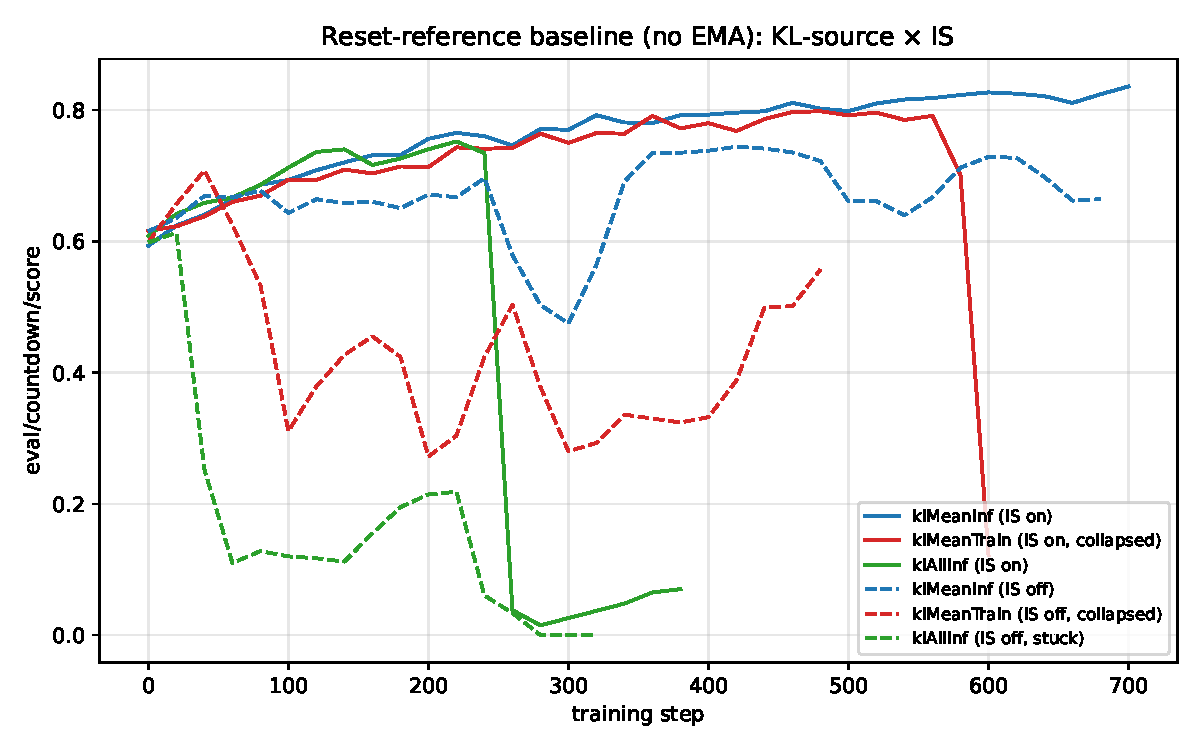
\includegraphics[width=0.95\linewidth]{fig_reset_baselines.pdf}
  \caption{Reset-reference (every $50$ steps) baseline. \texttt{klMeanInf} uses the inference snapshot for the K-group mean; \texttt{klMeanTrain} uses a live training-policy forward (which collapses around step $600$ with IS on, and around step $480$ with IS off); \texttt{klAllInf} also uses the inference snapshot for the per-sample KL term and gets stuck.}
  \label{fig:reset-baselines}
\end{figure}

The collapses with klMeanTrain centering were the original motivation for moving to EMA reference, on the hypothesis that an EMA reference would dampen the symmetric (live-train) centering term. The EMA matrix above shows that this dampening is not enough: klMeanTrain centering remains the worst configuration even with the EMA in place, suggesting the issue is the centering itself rather than the choice of reference policy.

\section{Approximation accuracy}

Figure~\ref{fig:approx-error} reports per-token error metrics between the first-order surrogate and the actual EMA-KL, computed inside \texttt{tba\_loss}: MAE, signed bias, raw relative error (with $\varepsilon=10^{-8}$), and relative error after clamping both quantities to $[-10,10]$. The metrics are over masked target tokens, averaged within each rollout.

\begin{figure}[ht]
  \centering
  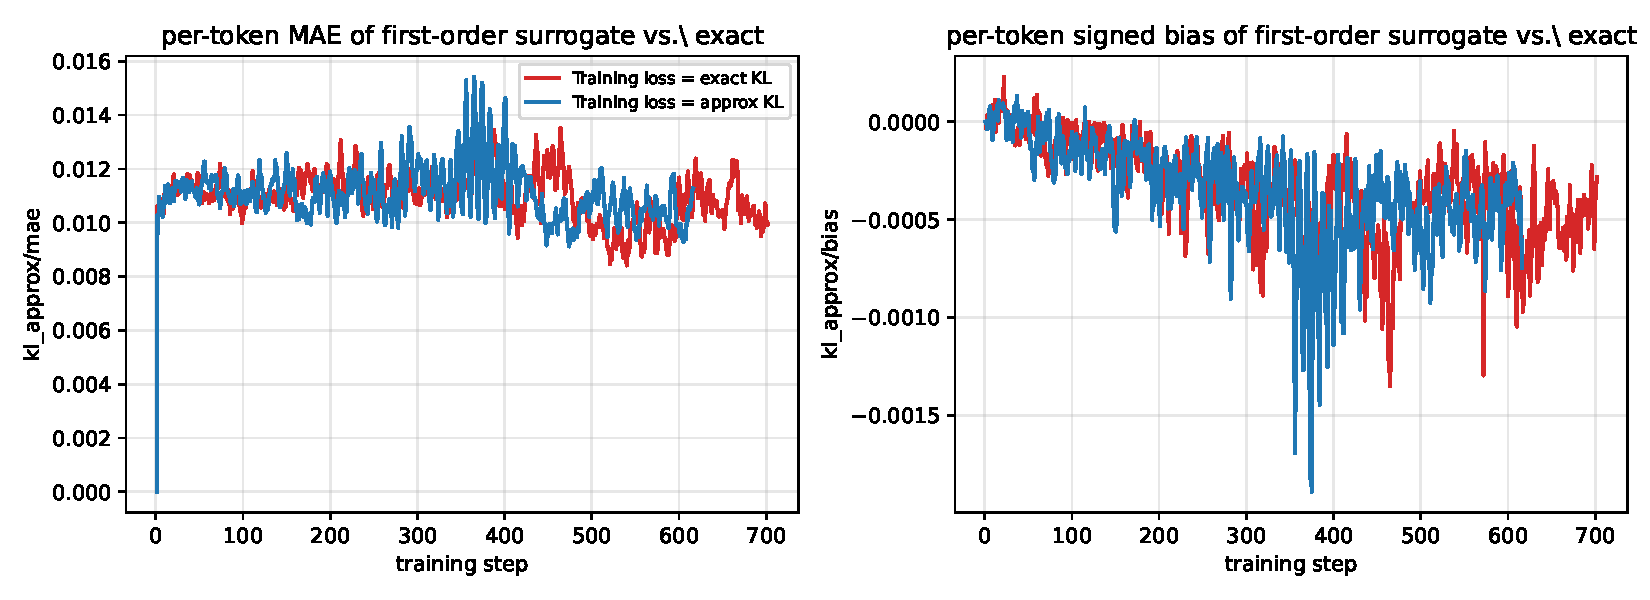
\includegraphics[width=0.98\linewidth]{fig_approx_error.pdf}
  \caption{Per-token error of the first-order surrogate against the exact EMA-KL, across training. MAE and signed bias are tightly bounded ($\sim\!10^{-2}$ and near-zero, respectively). The raw relative error is dominated by tokens where the actual KL is near zero, hence the spikes; the clamped variant tracks the signed-bias scale more closely.}
  \label{fig:approx-error}
\end{figure}

\paragraph{Reading the panels.}
\begin{itemize}[leftmargin=*]
  \item \emph{MAE} (top-left): consistently $\sim\!10^{-2}$ across all runs that have telemetry. The approximation is accurate at the per-token level over the full training trajectory.
  \item \emph{Bias} (top-right): tightly centered near zero, indicating the surrogate is unbiased under the locally-linear assumption of \texttt{main.tex}.
  \item \emph{Relative error} (bottom-left, log scale): occasionally spikes when the actual KL is near zero on most tokens, which is unavoidable for any ratio metric without a clamp.
  \item \emph{Clamped relative error} (bottom-right, log scale): clamping inputs to $[-10,10]$ before forming the ratio bounds the spikes; the resulting curve sits in the same low-$10^{-1}$ band as the bias-to-MAE ratio.
\end{itemize}

\section{Conclusions}

The first-order EMA-KL surrogate is empirically faithful to the exact EMA-KL: both deliver matching learning curves and final eval scores when used with no centering. The dominant variable in this experiment is not exact-vs-approx, but \emph{centering vs.\ no-centering}: klMeanTrain-style centering destabilizes training under both reference choices (reset and EMA), while no-centering yields the strongest results. This frees us to use the cheap surrogate in production without an additional reference forward pass, while leaving the question of useful centering schemes open.

\end{document}
